\documentclass[a4paper,10pt]{article}
\usepackage[]{graphicx}
\usepackage{subfigure}
\usepackage[]{times}
\usepackage{geometry}
\usepackage{cite}
\usepackage{framed}
\usepackage{hyperref}

\geometry{verbose,a4paper,tmargin=1.5cm,bmargin=2cm,lmargin=2cm,rmargin=2cm}
\renewcommand{\baselinestretch}{1.0}

\title{CADI user manual \\ \small (version 3.1)}

\author{
GICI group \vspace{0.1cm} \\
\small Department of Information and Communications Engineering \\
\small Universitat Aut{\`o}noma Barcelona \\
\small http://www.gici.uab.es  -  http://www.gici.uab.es/CADI \\
}

\date{\today}

\hyphenation{CADIServer}
\hyphenation{CADIClient}
\hyphenation{CADIViewer}
\hyphenation{CADIProxy}

\begin{document}

\maketitle
\begin{figure}
	\centering
	\subfigure{
   		
\includegraphics[scale=0.4] {images/logoUAB.png}
 	}
 	\hspace*{0.2\textwidth}
 	~\subfigure{
   		
\includegraphics[scale=0.4] {images/logoGICI.png}
 	}
 	\hspace*{0.2\textwidth}
 	~\subfigure{
   		
\includegraphics[scale=0.4] {images/logoDEIC.png}
 	}
\end{figure}
\thispagestyle{empty}
\newpage

\tableofcontents
\newpage


%%%%%%%%%%%%%%%%%%%%%%%%%%%%%%%%%%%%%%%%%%%%%%%%%%%%%%%%%%%%%%%%%%%%%%%%%%%%%%%
\section{Overview}
\label{sect:overview}

CADI is an implementation of the JPEG2000 Interactive Protocol (Part 9) standard.
Since the JPIP protocol is a client-server protocol, CADI is composed of four
applications: CADIServer (that implements a JPIP server), CADIViewer (implmenting
a Graphical User Interface for the JPIP client side), CADIClient (implementing
a JPIP client), and CADIProxy (that implments a JPIP proxy). All applications
are encapsulated in jar files in the \emph{dist/} directory and can be executed
separately using the JVM. 

The implementation provides the basic functionalities of the JPIP protocol, Basic
Communications Profile, and several capabilities of the Enhanded  Communication
Profile.
 
The source code of CADI has been designed and programmed with the aim to provide
a flexible framework, allowing users to easily integrate their modules to test
and develop new ideas inside the JPIP protocol in a easy way.

All applications, except for CADIViewer, provide different functionalities that
can be controlled via their command line parameters, they are passed as program
arguments. Each one of these parameters and their valid arguments will be
detailed in the section devoted to each of the four applications.


A development	manual is also available and the API is well documented
to facilitate an easy understanding, extension and modification of
the application. All the design and implementation details are widely
explained in these manuals and the source code is commented. All
these information is publicly available in the web page
http://www.gici.uab.es/CADI, where you can download the sources and
the manuals. To guarantee a free distribution, CADI has the General
Public License (GNU GPL) of the Free Software Foundation
(http://www.fsf.org/licensing/licenses/gpl.html).  

We have tried to make a good design and efforts have been made to
develop and implement the application as useful as
desirable. However, we could not foresee all the needs of CADI
users, so we will thank you for all the suggestions and comments
that you can report to us (gici-dev@deic.uab.es). 

\flushright{We hope you enjoy it, \vspace{0.25cm}\\GICI group}\flushleft{} 


\newpage
%%%%%%%%%%%%%%%%%%%%%%%%%%%%%%%%%%%%%%%%%%%%%%%%%%%%%%%%%%%%%%%%%%%%%%%%%%%%%%%
\section{CADIServer}
\label{sect:server}

The CADIServer application implements the server side of the JPIP protocol,
allowing JPIP clients to download JPEG2000 images.

CADIServer does not have a graphical interface and it must be launched from the
command line. Since the \emph{CADIServer.jar} is in the \emph{dist/} directory,
the following command {\tt java -jar dist/CADIServer.jar} will launch the server
using the default options (see section \ref{sect:server_parameters} for
detailed options).

\subsection{CADIServer parameters}
\label{sect:server_parameters}

In this section all supported parameters for the server command line are explained.
For a detailed description of each element in the table displayed for each parameter,
please see \ref{sect:annex_parameters}.


\begin{center}\begin{tabular}{|rr|rl|rl|}
\hline
\multicolumn{2}{|l|}{\textbf{$-$$-$ports}} & \multicolumn{4}{|l|}{$\{$int$[$int $[$int $[$ ...$]$$]$$]$$\}$} \\
\cline{3-6}
\multicolumn{2}{|l|}{\textbf{$-$p}} & \emph{Mandatory:} & No & \emph{Max reps:} & 1 \\
\hline
\emph{Explanation:} & \multicolumn{5}{|p{12cm}|}{Ports where server will listen to the client request.} \\
\hline
\emph{Default:} & \multicolumn{5}{|p{12cm}|}{80} \\
\hline
\end{tabular}\end{center}

\begin{center}\begin{tabular}{|rr|rl|rl|}
\hline
\multicolumn{2}{|l|}{\textbf{$-$$-$numThreads}} & \multicolumn{4}{|l|}{$\{$int$\}$} \\
\cline{3-6}
\multicolumn{2}{|l|}{\textbf{$-$nt}} & \emph{Mandatory:} & No & \emph{Max reps:} & 1 \\
\hline
\emph{Explanation:} & \multicolumn{5}{|p{12cm}|}{Number of threads that will be launched to process the request.} \\
\hline
\emph{Default:} & \multicolumn{5}{|p{12cm}|}{1} \\
\hline
\end{tabular}\end{center}

\begin{center}\begin{tabular}{|rr|rl|rl|}
\hline
\multicolumn{2}{|l|}{\textbf{$-$$-$targetsPath}} & \multicolumn{4}{|l|}{$\{$string$\}$} \\
\cline{3-6}
\multicolumn{2}{|l|}{\textbf{$-$tp}} & \emph{Mandatory:} & No & \emph{Max reps:} & 1 \\
\hline
\emph{Explanation:} & \multicolumn{5}{|p{12cm}|}{Root directory where the targets (image files) are stored. Default value is the directory where the server is launched.} \\
\hline
\emph{Default:} & \multicolumn{5}{|p{12cm}|}{} \\
\hline
\end{tabular}\end{center}

\begin{center}\begin{tabular}{|rr|rl|rl|}
\hline
\multicolumn{2}{|l|}{\textbf{$-$$-$logFile}} & \multicolumn{4}{|l|}{$\{$string$\}$} \\
\cline{3-6}
\multicolumn{2}{|l|}{\textbf{$-$lf}} & \emph{Mandatory:} & No & \emph{Max reps:} & 1 \\
\hline
\emph{Explanation:} & \multicolumn{5}{|p{12cm}|}{File where logs are saved.} \\
\hline
\emph{Default:} & \multicolumn{5}{|p{12cm}|}{} \\
\hline
\end{tabular}\end{center}
\begin{center}\begin{tabular}{|rr|rl|rl|}
\hline
\multicolumn{2}{|l|}{\textbf{$-$$-$logXML}} & \multicolumn{4}{|l|}{$\{$boolean$\}$} \\
\cline{3-6}
\multicolumn{2}{|l|}{\textbf{$-$lx}} & \emph{Mandatory:} & No & \emph{Max reps:} & 1 \\
\hline
\emph{Explanation:} & \multicolumn{5}{|p{12cm}|}{XML format is used in the log file. Value is a boolean: 0 indicates simple file format is used and 1 indicates XML format is used.} \\
\hline
\emph{Default:} & \multicolumn{5}{|p{12cm}|}{0} \\
\hline
\end{tabular}\end{center}

\begin{center}\begin{tabular}{|rr|rl|rl|}
\hline
\multicolumn{2}{|l|}{\textbf{$-$$-$logEnabled}} & \multicolumn{4}{|l|}{$\{$boolean$\}$} \\
\cline{3-6}
\multicolumn{2}{|l|}{\textbf{$-$le}} & \emph{Mandatory:} & No & \emph{Max reps:} & 1 \\
\hline
\emph{Explanation:} & \multicolumn{5}{|p{12cm}|}{Enables or disables the log. See the "-ll" parameter for more information about the detail level of logs.} \\
\hline
\emph{Default:} & \multicolumn{5}{|p{12cm}|}{} \\
\hline
\end{tabular}\end{center}

\begin{center}\begin{tabular}{|rr|rl|rl|}
\hline
\multicolumn{2}{|l|}{\textbf{$-$$-$logLevel}} & \multicolumn{4}{|l|}{$\{$int$\}$} \\
\cline{3-6}
\multicolumn{2}{|l|}{\textbf{$-$ll}} & \emph{Mandatory:} & No & \emph{Max reps:} & 1 \\
\hline
\emph{Explanation:} & \multicolumn{5}{|p{12cm}|}{Is the severity of the messages which will be logged. The "-le" parameter is set automatically. Available values are:\newline	2- logs informative messages\newline	3- logs warning messages\newline	4- logs error messages\newline when a log level is set, all upper levels are automatically set but lower severity messages are filtered.} \\
\hline
\emph{Default:} & \multicolumn{5}{|p{12cm}|}{2} \\
\hline
\end{tabular}\end{center}

\begin{center}\begin{tabular}{|rr|rl|rl|}
\hline
\multicolumn{2}{|l|}{\textbf{$-$$-$cacheDirectory}} & \multicolumn{4}{|l|}{$\{$string$\}$} \\
\cline{3-6}
\multicolumn{2}{|l|}{\textbf{$-$cd}} & \emph{Mandatory:} & No & \emph{Max reps:} & 1 \\
\hline
\emph{Explanation:} & \multicolumn{5}{|p{12cm}|}{Directory used as a temporal directory to save the cache data (not implemented yet).} \\
\hline
\emph{Default:} & \multicolumn{5}{|p{12cm}|}{} \\
\hline
\end{tabular}\end{center}
\begin{center}\begin{tabular}{|rr|rl|rl|}
\hline
\multicolumn{2}{|l|}{\textbf{$-$$-$deliveringMode}} & \multicolumn{4}{|l|}{$\{$int$\}$} \\
\cline{3-6}
\multicolumn{2}{|l|}{\textbf{$-$dm}} & \emph{Mandatory:} & No & \emph{Max reps:} & 1 \\
\hline
\emph{Explanation:} & \multicolumn{5}{|p{12cm}|}{Indicates the rate distortion method which is used in a JPEG2000 image to calculate de Window Of Interest. Available values are:\newline	1- precinct data are delivered layer by layer just as they appear in the codestream\newline	 2- the CPI method is uses to calculate the WOI. It only can be used with request that belongs to a session.\newline	3- the CoRD method is uses to calculate the WOI.\newline	4- applies a window scaling factor to each precinct to be delivered consisting on the overlap factor of each precinct with the window of interest requested.\newline OBS: Option 3 has been temporary disabled.} \\
\hline
\emph{Default:} & \multicolumn{5}{|p{12cm}|}{4} \\
\hline
\end{tabular}\end{center}

\begin{center}\begin{tabular}{|rr|rl|rl|}
\hline
\multicolumn{2}{|l|}{\textbf{$-$$-$cpiType}} & \multicolumn{4}{|l|}{$\{$int$\}$} \\
\cline{3-6}
\multicolumn{2}{|l|}{\textbf{$-$cpit}} & \emph{Mandatory:} & No & \emph{Max reps:} & 1 \\
\hline
\emph{Explanation:} & \multicolumn{5}{|p{12cm}|}{Indicates, within the CPI rate-distortion method, the subtype which will be used to delivery the requested WOI. This parameter must be only available when the rate-distortion (-rd) parameter is 2. Otherwise, it won't be taken into account. Available values are:\newline	1- Only one packet for each precinct is generated. Therefore, delivered image has only one quality layer.\newline	2- Creates one packet per each bit plane. Therefore, delivered image has as quality layers as number of bit planes.\newline	3- Creates one packet per each coding pass. Therefore, delivered image has as quality layers as number of coding passes.\newline 4- Images are delivered following the SCALE method.\newline This parameter is only allowd if the "-dm" parameter is 2.} \\
\hline
\emph{Default:} & \multicolumn{5}{|p{12cm}|}{0} \\
\hline
\end{tabular}\end{center}
\begin{center}\begin{tabular}{|rr|rl|rl|}
\hline
\multicolumn{2}{|l|}{\textbf{$-$$-$cordType}} & \multicolumn{4}{|l|}{$\{$int$\}$} \\
\cline{3-6}
\multicolumn{2}{|l|}{\textbf{$-$cordt}} & \emph{Mandatory:} & No & \emph{Max reps:} & 1 \\
\hline
\emph{Explanation:} & \multicolumn{5}{|p{12cm}|}{Indicates, within the CPI rate-distortion method, the subtype which will be used to delivery the requested WOI. This parameter must be only available when the rate-distortion (-rd) parameter is 2. Otherwise, it won't be taken into account. Available values are:\newline	1- Is the classic CoRD algorithm.\newline	2- Is a modification of the CoRD algorithm in order to reduce the overhead of packet and JPIP message headers.\newline This parameter is only allowd if the "-dm" parameter is 3.} \\
\hline
\emph{Default:} & \multicolumn{5}{|p{12cm}|}{0} \\
\hline
\end{tabular}\end{center}

\begin{center}\begin{tabular}{|rr|rl|rl|}
\hline
\multicolumn{2}{|l|}{\textbf{$-$$-$deliveryProgressionOrder}} & \multicolumn{4}{|l|}{$\{$int$\}$} \\
\cline{3-6}
\multicolumn{2}{|l|}{\textbf{$-$dpo}} & \emph{Mandatory:} & No & \emph{Max reps:} & 1 \\
\hline
\emph{Explanation:} & \multicolumn{5}{|p{12cm}|}{Indicates the progression order which will be used to delivery data. If this parameter is not set, the progression order of the codestream will be used. Otherwise, the progression order of the codestream will not be taken into account. Available values are:\newline	0- Layer-Resolution-Component-Position (LRCP).\newline	1- Resolution-Layer-Component-Position (RLCP).\newline	 2- Resolution-Position-Component-Layer (RPCL).\newline	 3- Position-Component-Resolution-Layer (PCRL).\newline 	4- Component-Position-Resolution-Layer (CPRL).\newline This parameter is only allowed if the "-dm" parameter is 1.} \\
\hline
\emph{Default:} & \multicolumn{5}{|p{12cm}|}{} \\
\hline
\end{tabular}\end{center}
\begin{center}\begin{tabular}{|rr|rl|rl|}
\hline
\multicolumn{2}{|l|}{\textbf{$-$$-$keepAliveTiemout}} & \multicolumn{4}{|l|}{$\{$int$\}$} \\
\cline{3-6}
\multicolumn{2}{|l|}{\textbf{$-$kt}} & \emph{Mandatory:} & No & \emph{Max reps:} & 1 \\
\hline
\emph{Explanation:} & \multicolumn{5}{|p{12cm}|}{Specifies the timeout (in milliseconds) that the socket is kept opened and waiting for new client requests.} \\
\hline
\emph{Default:} & \multicolumn{5}{|p{12cm}|}{1} \\
\hline
\end{tabular}\end{center}
\begin{center}\begin{tabular}{|rr|rl|rl|}
\hline
\multicolumn{2}{|l|}{\textbf{$-$$-$maxRate}} & \multicolumn{4}{|l|}{$\{$int$\}$} \\
\cline{3-6}
\multicolumn{2}{|l|}{\textbf{$-$mr}} & \emph{Mandatory:} & No & \emph{Max reps:} & 1 \\
\hline
\emph{Explanation:} & \multicolumn{5}{|p{12cm}|}{Specifies the maximum rate (bytes per second) which will be used to delivery data (0 means unlimited).} \\
\hline
\emph{Default:} & \multicolumn{5}{|p{12cm}|}{0} \\
\hline
\end{tabular}\end{center}
\begin{center}\begin{tabular}{|rr|rl|rl|}
\hline
\multicolumn{2}{|l|}{\textbf{$-$$-$trafficShaping}} & \multicolumn{4}{|l|}{$\{$int$\}$} \\
\cline{3-6}
\multicolumn{2}{|l|}{\textbf{$-$ts}} & \emph{Mandatory:} & No & \emph{Max reps:} & 1 \\
\hline
\emph{Explanation:} & \multicolumn{5}{|p{12cm}|}{Allows to choose a trafic shaping algorithm. Allowed values are:	0- None algoritm is applied.	1- The token-bucket algoritm is applied. Data are transmitted at the constant rate fixed by the "-mr" parameter rate, but it also allows data busts.	2- The leaky-bucket algoritm is applied. Data are delivered at the constant rate defined in the "-mr" option.OBS: This parameter requires the "-mr" parameter.} \\
\hline
\emph{Default:} & \multicolumn{5}{|p{12cm}|}{0} \\
\hline
\end{tabular}\end{center}
\begin{center}\begin{tabular}{|rr|rl|rl|}
\hline
\multicolumn{2}{|l|}{\textbf{$-$$-$independentMessageHeaders}} & \multicolumn{4}{|l|}{$\{$booelan$\}$} \\
\cline{3-6}
\multicolumn{2}{|l|}{\textbf{$-$imh}} & \emph{Mandatory:} & No & \emph{Max reps:} & 1 \\
\hline
\emph{Explanation:} & \multicolumn{5}{|p{12cm}|}{Indicates which form of JPIP messsage headers will be used (independent or dependent). The independent form is a long form where the message headers are completely self-describing. Meanwhile, the depenent form message headers make use of information in the headers of previous messages. The dependent form makes a shorter message header than the independent form, but sequence ordering of received message must be taken into account.} \\
\hline
\emph{Default:} & \multicolumn{5}{|p{12cm}|}{1} \\
\hline
\end{tabular}\end{center}
\begin{center}\begin{tabular}{|rr|rl|rl|}
\hline
\multicolumn{2}{|l|}{\textbf{$-$$-$predictiveModel}} & \multicolumn{4}{|l|}{$\{$boolean$\}$} \\
\cline{3-6}
\multicolumn{2}{|l|}{\textbf{$-$pm}} & \emph{Mandatory:} & No & \emph{Max reps:} & 1 \\
\hline
\emph{Explanation:} & \multicolumn{5}{|p{12cm}|}{This parameter indicates that a predictive model can be applied in the image delivering. The predictive model to be applied is read from a text file whose name is the same as the compressed image but with the extension "pm". The file must have a line for each spatial region (precinct) with the following format "precinct\_id value", where the precinct\_id is the unique precinct identifier defined in the JPIP protocol and the value is a real number in the range [0, 1] with the relevance of the relevance of the precinct. The remainder precincts not included in the file will be considered with relevance 0. And if the beginning-of-line character is an \#, it is considered a comment and ignored.This parameter is only allowed if the "-dm" parameter is 4.
} \\
\hline
\emph{Default:} & \multicolumn{5}{|p{12cm}|}{0} \\
\hline
\end{tabular}\end{center}
\begin{center}\begin{tabular}{|rr|rl|rl|}
\hline
\multicolumn{2}{|l|}{\textbf{$-$$-$help}} & \multicolumn{4}{|l|}{} \\
\cline{3-6}
\multicolumn{2}{|l|}{\textbf{$-$h}} & \emph{Mandatory:} & No & \emph{Max reps:} & 1 \\
\hline
\emph{Explanation:} & \multicolumn{5}{|p{12cm}|}{Displays this help and exits program.} \\
\hline
\emph{Default:} & \multicolumn{5}{|p{12cm}|}{} \\
\hline
\end{tabular}\end{center}
\begin{center}\begin{tabular}{|rr|rl|rl|}
\hline
\multicolumn{2}{|l|}{\textbf{$-$$-$warranty}} & \multicolumn{4}{|l|}{} \\
\cline{3-6}
\multicolumn{2}{|l|}{\textbf{$-$w}} & \emph{Mandatory:} & No & \emph{Max reps:} & 1 \\
\hline
\emph{Explanation:} & \multicolumn{5}{|p{12cm}|}{} \\
\hline
\emph{Default:} & \multicolumn{5}{|p{12cm}|}{} \\
\hline
\end{tabular}\end{center}
\begin{center}\begin{tabular}{|rr|rl|rl|}
\hline
\multicolumn{2}{|l|}{\textbf{$-$$-$liability}} & \multicolumn{4}{|l|}{} \\
\cline{3-6}
\multicolumn{2}{|l|}{\textbf{$-$l}} & \emph{Mandatory:} & No & \emph{Max reps:} & 1 \\
\hline
\emph{Explanation:} & \multicolumn{5}{|p{12cm}|}{} \\
\hline
\emph{Default:} & \multicolumn{5}{|p{12cm}|}{} \\
\hline
\end{tabular}\end{center}
\begin{center}\begin{tabular}{|rr|rl|rl|}
\hline
\multicolumn{2}{|l|}{\textbf{$-$$-$copyright}} & \multicolumn{4}{|l|}{} \\
\cline{3-6}
\multicolumn{2}{|l|}{\textbf{$-$c}} & \emph{Mandatory:} & No & \emph{Max reps:} & 1 \\
\hline
\emph{Explanation:} & \multicolumn{5}{|p{12cm}|}{} \\
\hline
\emph{Default:} & \multicolumn{5}{|p{12cm}|}{} \\
\hline
\end{tabular}\end{center}



%%%%%%%%%%%%%%%%%%%%%%%%%%%%%%%%%%%%%%%%%%%%%%%%%%%%%%%%%%%%%%%%%%%%%%%%%%%%%%%
\subsection{Examples}
\label{sect:examples}

Some basic examples of CADIServer usage and combination of the different options
of the command line parameters are shown in this section.

\begin{itemize}
	\item Launch the server with the default options. Server is listening to in the
	port 80, the current directory is the path where images must be placed, it
	launches as threads as number of processors, and it uses the Window Scaling
	Factor as strategy for delivering images.
	\begin{framed}
	\texttt{\$java -jar dist/CADIServer.jar}
	\end{framed}

	\item Display the help information.
	\begin{framed}
	\texttt{\$java -jar dist/CADIServer.jar -h}
	\end{framed}
	
	\item Launch the server listening to on por 2080.
	\begin{framed}
	\texttt{\$java -jar dist/CADIServer.jar -p 2080}
	\end{framed}
	
	\item Change the root path from where images (targets) are red to the \emph{workDir} directory.
	\begin{framed}
	\texttt{\$java -jar dist/CADIServer.jar -tp workDir}
	\end{framed}

	\item Change the rate-distortion algorithm used to deliver images.
	\begin{framed}
	\texttt{\$java -jar dist/CADIServer.jar -rd 2}
	\end{framed}
	
	\item Adjust the maximum rate images are delivering (10KB) and set the 
	the token-backut as traffic shaping algorithm.
	\begin{framed}
	\texttt{\$java -jar dist/CADIServer.jar -ts 1 -mr 10000}
	\end{framed}
	
\end{itemize}




\newpage
%%%%%%%%%%%%%%%%%%%%%%%%%%%%%%%%%%%%%%%%%%%%%%%%%%%%%%%%%%%%%%%%%%%%%%%%%%%%%%%
\section{CADIClient}
\label{sect:client}

The CADI client application implements the client side of the JPIP protocol. It
is a command line application to get images from a JPIP server and save them
in a file.

Session cannot be used!.

\subsection{CADIClient parameters}
\label{sect:client_parameters}
In this section all supported parameters for the server command line are explained.
For a detailed description of each element in the table displayed for each parameter,
please see \ref{sect:annex_parameters}.


CADIClient version 3.1

\begin{center}\begin{tabular}{|rr|rl|rl|}
\hline
\multicolumn{2}{|l|}{\textbf{$-$$-$server}} & \multicolumn{4}{|l|}{$\{$string$\}$} \\
\cline{3-6}
\multicolumn{2}{|l|}{\textbf{$-$s}} & \emph{Mandatory:} & No & \emph{Max reps:} & 1 \\
\hline
\emph{Explanation:} & \multicolumn{5}{|p{12cm}|}{Server name where the image to be retrieved is.} \\
\hline
\emph{Default:} & \multicolumn{5}{|p{12cm}|}{localhost} \\
\hline
\end{tabular}\end{center}
\begin{center}\begin{tabular}{|rr|rl|rl|}
\hline
\multicolumn{2}{|l|}{\textbf{$-$$-$port}} & \multicolumn{4}{|l|}{$\{$int$\}$} \\
\cline{3-6}
\multicolumn{2}{|l|}{\textbf{$-$p}} & \emph{Mandatory:} & No & \emph{Max reps:} & 1 \\
\hline
\emph{Explanation:} & \multicolumn{5}{|p{12cm}|}{Port number where the server is listening to client requests.} \\
\hline
\emph{Default:} & \multicolumn{5}{|p{12cm}|}{80} \\
\hline
\end{tabular}\end{center}
\begin{center}\begin{tabular}{|rr|rl|rl|}
\hline
\multicolumn{2}{|l|}{\textbf{$-$$-$proxyServer}} & \multicolumn{4}{|l|}{$\{$string$\}$} \\
\cline{3-6}
\multicolumn{2}{|l|}{\textbf{$-$ps}} & \emph{Mandatory:} & No & \emph{Max reps:} & 1 \\
\hline
\emph{Explanation:} & \multicolumn{5}{|p{12cm}|}{Server name where the image to be retrieved is.} \\
\hline
\emph{Default:} & \multicolumn{5}{|p{12cm}|}{} \\
\hline
\end{tabular}\end{center}
\begin{center}\begin{tabular}{|rr|rl|rl|}
\hline
\multicolumn{2}{|l|}{\textbf{$-$$-$proxyPort}} & \multicolumn{4}{|l|}{$\{$int$\}$} \\
\cline{3-6}
\multicolumn{2}{|l|}{\textbf{$-$pp}} & \emph{Mandatory:} & No & \emph{Max reps:} & 1 \\
\hline
\emph{Explanation:} & \multicolumn{5}{|p{12cm}|}{Port number where the server is listening to client requests.} \\
\hline
\emph{Default:} & \multicolumn{5}{|p{12cm}|}{8080} \\
\hline
\end{tabular}\end{center}
\begin{center}\begin{tabular}{|rr|rl|rl|}
\hline
\multicolumn{2}{|l|}{\textbf{$-$$-$target}} & \multicolumn{4}{|l|}{$\{$string$\}$} \\
\cline{3-6}
\multicolumn{2}{|l|}{\textbf{$-$t}} & \emph{Mandatory:} & No & \emph{Max reps:} & 1 \\
\hline
\emph{Explanation:} & \multicolumn{5}{|p{12cm}|}{Targets to be retrieved from the server. If this parameter is not set, the uri ("-u") parameter must be appear.} \\
\hline
\emph{Default:} & \multicolumn{5}{|p{12cm}|}{} \\
\hline
\end{tabular}\end{center}
\begin{center}\begin{tabular}{|rr|rl|rl|}
\hline
\multicolumn{2}{|l|}{\textbf{$-$$-$uri}} & \multicolumn{4}{|l|}{$\{$string$\}$} \\
\cline{3-6}
\multicolumn{2}{|l|}{\textbf{$-$u}} & \emph{Mandatory:} & No & \emph{Max reps:} & 1 \\
\hline
\emph{Explanation:} & \multicolumn{5}{|p{12cm}|}{Is an Uniform Resource Identifier of the target to be retrieved. If this parameter is not set, the target ("-t") parameter must be appear.} \\
\hline
\emph{Default:} & \multicolumn{5}{|p{12cm}|}{} \\
\hline
\end{tabular}\end{center}
\begin{center}\begin{tabular}{|rr|rl|rl|}
\hline
\multicolumn{2}{|l|}{\textbf{$-$$-$outputImage}} & \multicolumn{4}{|l|}{$\{$string$\}$} \\
\cline{3-6}
\multicolumn{2}{|l|}{\textbf{$-$o}} & \emph{Mandatory:} & Yes & \emph{Max reps:} & $\infty$ \\
\hline
\emph{Explanation:} & \multicolumn{5}{|p{12cm}|}{Output image file name where recovered image samples will be stored. Image file type will be decided depending on the extension. Valid file types are:\newline RAW/IMG raw data (if outputImage is raw data, "-og" argument is mandatory)\newline PNM/PGM/PPM PGM is used when image have 1 component, PPM when there are 3 components and PNM for both\newline TIFF\newline JPEG (not recommended because it degenerates recovered image)\newline BMP (not recommended)\newline ATTENTION: if recovered image samples are signed only RAW/IMG data with a signed data type will preserve image samples consistently. Using other file format will cause image data damages.} \\
\hline
\emph{Default:} & \multicolumn{5}{|p{12cm}|}{} \\
\hline
\end{tabular}\end{center}
\begin{center}\begin{tabular}{|rr|rl|rl|}
\hline
\multicolumn{2}{|l|}{\textbf{$-$$-$ouputImageGeometry}} & \multicolumn{4}{|l|}{$\{$int int$\}$} \\
\cline{3-6}
\multicolumn{2}{|l|}{\textbf{$-$og}} & \emph{Mandatory:} & No & \emph{Max reps:} & 1 \\
\hline
\emph{Explanation:} & \multicolumn{5}{|p{12cm}|}{Image raw data type. Parameters are:\newline 1- data type. Possible values are:\newline   0- boolean (1 byte)\newline   1- unsigned int (1 byte)\newline   2- unsigned int (2 bytes)\newline   3- signed int (2 bytes)\newline   4- signed int (4 bytes)\newline   5- signed int (8 bytes)\newline   6- float (4 bytes)\newline   7- double (8 bytes)\newline 2- Byte order (0 if BIG ENDIAN, 1 if LITTLE ENDIAN)} \\
\hline
\emph{Default:} & \multicolumn{5}{|p{12cm}|}{} \\
\hline
\end{tabular}\end{center}
\begin{center}\begin{tabular}{|rr|rl|rl|}
\hline
\multicolumn{2}{|l|}{\textbf{$-$$-$compnents}} & \multicolumn{4}{|l|}{$\{$int$[$int $[$int $[$ ...$]$$]$$]$$\}$} \\
\cline{3-6}
\multicolumn{2}{|l|}{\textbf{$-$cs}} & \emph{Mandatory:} & No & \emph{Max reps:} & 1 \\
\hline
\emph{Explanation:} & \multicolumn{5}{|p{12cm}|}{Components of the image to be retrieved. This parameters is not compatible with the components ranges ("-cr") parameter} \\
\hline
\emph{Default:} & \multicolumn{5}{|p{12cm}|}{} \\
\hline
\end{tabular}\end{center}
\begin{center}\begin{tabular}{|rr|rl|rl|}
\hline
\multicolumn{2}{|l|}{\textbf{$-$$-$componentRanges}} & \multicolumn{4}{|l|}{$\{$int-int $[$int-int $[$int-int $[$ ...$]$$]$$]$$\}$} \\
\cline{3-6}
\multicolumn{2}{|l|}{\textbf{$-$cr}} & \emph{Mandatory:} & No & \emph{Max reps:} & 1 \\
\hline
\emph{Explanation:} & \multicolumn{5}{|p{12cm}|}{Ranges of components. This parameters is not compatible with the components ("-cr") parameter. \newline ATTENTION: This option is not implemented yet!} \\
\hline
\emph{Default:} & \multicolumn{5}{|p{12cm}|}{} \\
\hline
\end{tabular}\end{center}
\begin{center}\begin{tabular}{|rr|rl|rl|}
\hline
\multicolumn{2}{|l|}{\textbf{$-$$-$resolutionLevel}} & \multicolumn{4}{|l|}{$\{$int$\}$} \\
\cline{3-6}
\multicolumn{2}{|l|}{\textbf{$-$rl}} & \emph{Mandatory:} & No & \emph{Max reps:} & 1 \\
\hline
\emph{Explanation:} & \multicolumn{5}{|p{12cm}|}{Is the resolution level at which the image is retrieved. This parameter is not compatible with frame size ("-fs") parameter.} \\
\hline
\emph{Default:} & \multicolumn{5}{|p{12cm}|}{} \\
\hline
\end{tabular}\end{center}
\begin{center}\begin{tabular}{|rr|rl|rl|}
\hline
\multicolumn{2}{|l|}{\textbf{$-$$-$frameSize}} & \multicolumn{4}{|l|}{$\{$int int$\}$} \\
\cline{3-6}
\multicolumn{2}{|l|}{\textbf{$-$fs}} & \emph{Mandatory:} & No & \emph{Max reps:} & 1 \\
\hline
\emph{Explanation:} & \multicolumn{5}{|p{12cm}|}{Is the resolution level associate with the Window of Interest. The first value is the width, and the second one is the height. This parameter is not compatible with resolution level ("-rl") parameter.} \\
\hline
\emph{Default:} & \multicolumn{5}{|p{12cm}|}{} \\
\hline
\end{tabular}\end{center}
\begin{center}\begin{tabular}{|rr|rl|rl|}
\hline
\multicolumn{2}{|l|}{\textbf{$-$$-$regionOffset}} & \multicolumn{4}{|l|}{$\{$int int$\}$} \\
\cline{3-6}
\multicolumn{2}{|l|}{\textbf{$-$ro}} & \emph{Mandatory:} & No & \emph{Max reps:} & 1 \\
\hline
\emph{Explanation:} & \multicolumn{5}{|p{12cm}|}{Is the top-left coordinates of the Window of Interest. The first value is the left coordinate, and the second on is the top coordinate.} \\
\hline
\emph{Default:} & \multicolumn{5}{|p{12cm}|}{} \\
\hline
\end{tabular}\end{center}
\begin{center}\begin{tabular}{|rr|rl|rl|}
\hline
\multicolumn{2}{|l|}{\textbf{$-$$-$regionSize}} & \multicolumn{4}{|l|}{$\{$int int$\}$} \\
\cline{3-6}
\multicolumn{2}{|l|}{\textbf{$-$rs}} & \emph{Mandatory:} & No & \emph{Max reps:} & 1 \\
\hline
\emph{Explanation:} & \multicolumn{5}{|p{12cm}|}{Is the size of the Window of Interest. The first value is the width, and the second one is the height.} \\
\hline
\emph{Default:} & \multicolumn{5}{|p{12cm}|}{} \\
\hline
\end{tabular}\end{center}
\begin{center}\begin{tabular}{|rr|rl|rl|}
\hline
\multicolumn{2}{|l|}{\textbf{$-$$-$layers}} & \multicolumn{4}{|l|}{$\{$int$\}$} \\
\cline{3-6}
\multicolumn{2}{|l|}{\textbf{$-$ly}} & \emph{Mandatory:} & No & \emph{Max reps:} & 1 \\
\hline
\emph{Explanation:} & \multicolumn{5}{|p{12cm}|}{Specifies the maximum number of layers which will retrieved for the target.} \\
\hline
\emph{Default:} & \multicolumn{5}{|p{12cm}|}{0} \\
\hline
\end{tabular}\end{center}
\begin{center}\begin{tabular}{|rr|rl|rl|}
\hline
\multicolumn{2}{|l|}{\textbf{$-$$-$quality}} & \multicolumn{4}{|l|}{$\{$int$\}$} \\
\cline{3-6}
\multicolumn{2}{|l|}{\textbf{$-$q}} & \emph{Mandatory:} & No & \emph{Max reps:} & 1 \\
\hline
\emph{Explanation:} & \multicolumn{5}{|p{12cm}|}{Specifies the maximum quality which will retrieved for the target.\newline ATTENTION: This option is not implemented yet!} \\
\hline
\emph{Default:} & \multicolumn{5}{|p{12cm}|}{100} \\
\hline
\end{tabular}\end{center}
\begin{center}\begin{tabular}{|rr|rl|rl|}
\hline
\multicolumn{2}{|l|}{\textbf{$-$$-$roundDirection}} & \multicolumn{4}{|l|}{$\{$int$\}$} \\
\cline{3-6}
\multicolumn{2}{|l|}{\textbf{$-$rd}} & \emph{Mandatory:} & No & \emph{Max reps:} & 1 \\
\hline
\emph{Explanation:} & \multicolumn{5}{|p{12cm}|}{Specifies how the image resolution shall be selected. Allowed values:\newline  1- round-down\newline  2- round-up\newline  3- closest} \\
\hline
\emph{Default:} & \multicolumn{5}{|p{12cm}|}{1} \\
\hline
\end{tabular}\end{center}
\begin{center}\begin{tabular}{|rr|rl|rl|}
\hline
\multicolumn{2}{|l|}{\textbf{$-$$-$maxTargetLength}} & \multicolumn{4}{|l|}{$\{$int$\}$} \\
\cline{3-6}
\multicolumn{2}{|l|}{\textbf{$-$ml}} & \emph{Mandatory:} & No & \emph{Max reps:} & 1 \\
\hline
\emph{Explanation:} & \multicolumn{5}{|p{12cm}|}{Specifies the maximum amount of bytes the client wants the server to send in response to the client request.} \\
\hline
\emph{Default:} & \multicolumn{5}{|p{12cm}|}{0} \\
\hline
\end{tabular}\end{center}
\begin{center}\begin{tabular}{|rr|rl|rl|}
\hline
\multicolumn{2}{|l|}{\textbf{$-$$-$help}} & \multicolumn{4}{|l|}{} \\
\cline{3-6}
\multicolumn{2}{|l|}{\textbf{$-$h}} & \emph{Mandatory:} & No & \emph{Max reps:} & 1 \\
\hline
\emph{Explanation:} & \multicolumn{5}{|p{12cm}|}{Displays this help and exits program.} \\
\hline
\emph{Default:} & \multicolumn{5}{|p{12cm}|}{} \\
\hline
\end{tabular}\end{center}
\begin{center}\begin{tabular}{|rr|rl|rl|}
\hline
\multicolumn{2}{|l|}{\textbf{$-$$-$warranty}} & \multicolumn{4}{|l|}{} \\
\cline{3-6}
\multicolumn{2}{|l|}{\textbf{$-$w}} & \emph{Mandatory:} & No & \emph{Max reps:} & 1 \\
\hline
\emph{Explanation:} & \multicolumn{5}{|p{12cm}|}{} \\
\hline
\emph{Default:} & \multicolumn{5}{|p{12cm}|}{} \\
\hline
\end{tabular}\end{center}
\begin{center}\begin{tabular}{|rr|rl|rl|}
\hline
\multicolumn{2}{|l|}{\textbf{$-$$-$liability}} & \multicolumn{4}{|l|}{} \\
\cline{3-6}
\multicolumn{2}{|l|}{\textbf{$-$l}} & \emph{Mandatory:} & No & \emph{Max reps:} & 1 \\
\hline
\emph{Explanation:} & \multicolumn{5}{|p{12cm}|}{} \\
\hline
\emph{Default:} & \multicolumn{5}{|p{12cm}|}{} \\
\hline
\end{tabular}\end{center}
\begin{center}\begin{tabular}{|rr|rl|rl|}
\hline
\multicolumn{2}{|l|}{\textbf{$-$$-$copyright}} & \multicolumn{4}{|l|}{} \\
\cline{3-6}
\multicolumn{2}{|l|}{\textbf{$-$c}} & \emph{Mandatory:} & No & \emph{Max reps:} & 1 \\
\hline
\emph{Explanation:} & \multicolumn{5}{|p{12cm}|}{} \\
\hline
\emph{Default:} & \multicolumn{5}{|p{12cm}|}{} \\
\hline
\end{tabular}\end{center}


%%%%%%%%%%%%%%%%%%%%%%%%%%%%%%%%%%%%%%%%%%%%%%%%%%%%%%%%%%%%%%%%%%%%%%%%%%%%%%%
\subsection{Examples}
\label{sect:client_examples}

\begin{itemize}
	\item Display the help information.
	\begin{framed}
	\texttt{\$java -jar dist/CADIClient.jar -h}
	\end{framed}
	
	\item Request the image "image.jpc" from a JPIP server running on the local
machine on port 80. The downloaded image is saved in the file "output\_image.ppm".
	\begin{framed}
	\texttt{\$java -jar dist/CADIClient.jar -t image.jpc -o output\_image.ppm}
	\end{framed}
	
	\item Request the image "image.jpc" from a JPIP server running on the machine
	"jpipserver.domain" on port 9000. The downloaded image is saved in the file
	"output\_image.ppm".
	\begin{framed}
	\texttt{\$java -jar dist/CADIClient.jar -t image.jpc -s jpipserver.domain -p 9000 -o output\_image.ppm}
	\end{framed}
	
	\item Request the image "image.jpc" from a JPIP server running on the machine
	"jpipserver.domain" on port 9000 through a JPIP proxy that is running on the machine "jpipproxy.domain" on port 8080.
	\begin{framed}
	\texttt{\$java -jar dist/CADIClient.jar -t image.jpc -s jpipserver.domain -p 9000 -ps jpipproxy.domain -pp 8080 -o output\_image.ppm}
	\end{framed}
	
	\item Request a window/region of the image. The client requests for 10 layers
	of a region of the image "image.jpc" defined by the frame size of
	5000$\times$4000 pixels located at position 1000$\times$1000 and size
	1024$\times$768.
	\begin{framed}
	\texttt{\$java -jar dist/CADIClient.jar -t image.jpc -fs 5000 4000 -ro 1000 1000 -rs 1024 768 -ly 10 -o output\_image.ppm}
	\end{framed}

\end{itemize}


\newpage
%%%%%%%%%%%%%%%%%%%%%%%%%%%%%%%%%%%%%%%%%%%%%%%%%%%%%%%%%%%%%%%%%%%%%%%%%%%%%%%
\section{CADIViewer}
\label{sect:viewer}

The CADIViewer application is a Graphical User Interface of the CADI client.\\
\vspace*{0.5cm}
Once the CADIViewer has been launched ({\tt java -jar dist/CADIViewer.jar})
next window will be displayed.
\begin{figure}[!h]
	\centering
	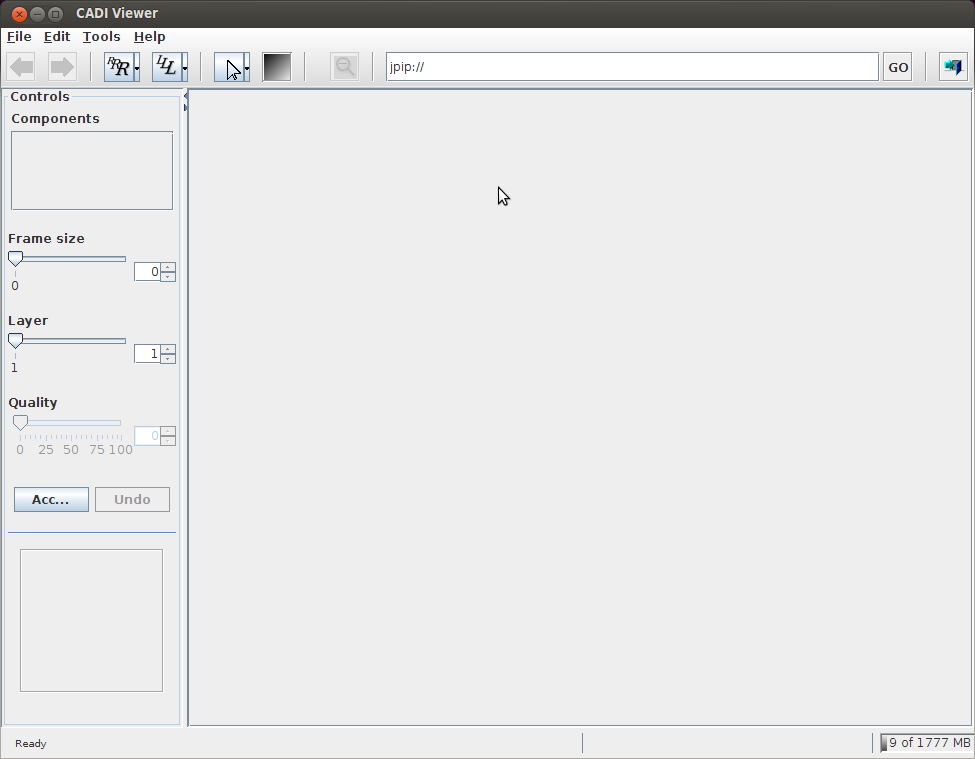
\includegraphics[scale=0.4]{images/CADIViewer-screenshot-ini.png} \\
\end{figure}
\vspace*{0.5cm}

Next step is to open a new session through the menu \emph{File $>$ New Session}
or by means of the shortcut \emph{Alt+N}. It will open a New Session Dialog window.
\begin{figure}[!h]
	\centering
	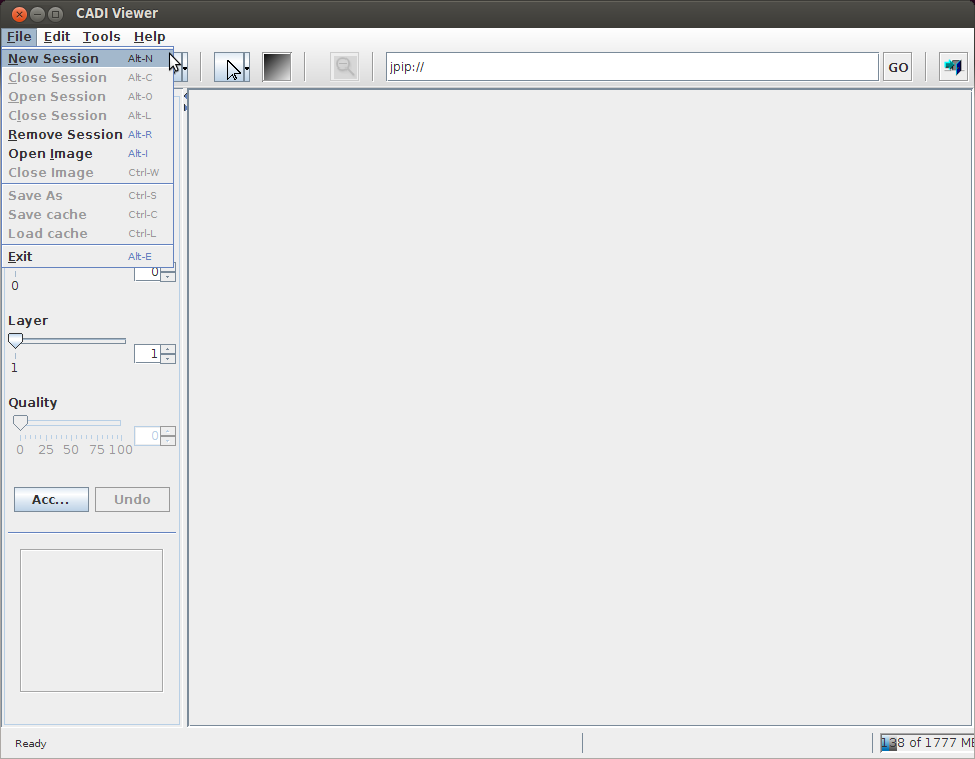
\includegraphics[scale=0.4]{images/CADIViewer-screenshot-MenuFile.png} \\
\end{figure}
\vspace*{0.5cm}

In the \emph{New Session Dialog} window there are two sections: JPIP server and
Proxy server. Only parameters in the JPIP server are mandatory. Then, the
\emph{Target} is the JPEG2000 image to be requested, the \emph{Host} is the 
server where the JPIP server is running on, and the \emph{Port} is the port on where
the JPIP server is listening to. Regarding the Proxy server section, the 
\emph{Host} is the server name where the JPIP proxy is running on, and the
\emph{Port} is the port of the JPIP proxy. Moreover, advanced preferences
can be configured if click \emph{Preferences} button.
button 
\begin{figure}[!h]
	\centering
	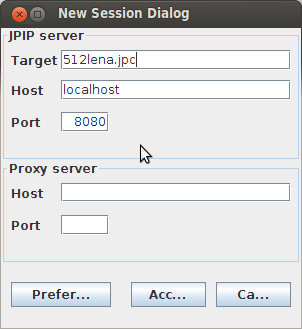
\includegraphics[scale=0.4]{images/CADIViewer-screenshot-NewSessionDialog.png} \\
\end{figure}
\vspace*{0.5cm}

The \emph{Preferences dialog window} is opened if the \emph{Preference} boton has
been clicked. In this dialog window prefences are grouped in three tabs.
\emph{Session type} allows to configure the connection to the JPIP server using
Statless or Stateful sessions (only Sessions over HTTP are available). Stateful
connections are recommended because they reduce the amount of data to be sent
to the server.
\begin{figure}[!h]
	\centering
	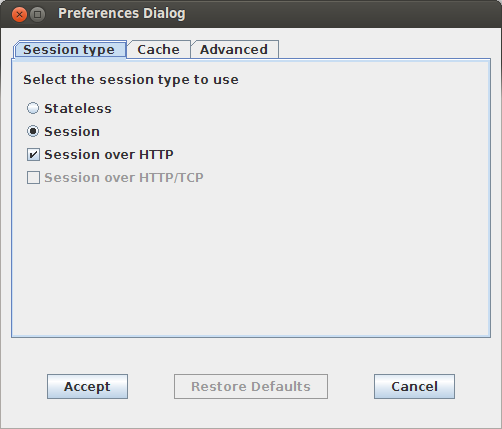
\includegraphics[scale=0.4]{images/CADIViewer-screenshot-PreferencesDialog_SessionType.png} \\
\end{figure}
\vspace*{0.5cm}

The tab \emph{Cache} in the \emph{Preferences dialog window} allows to configure
the type of cache to be used in the client or not to use cache. Each type of cache
can be qualified to be more precise in the type to use. \\
\begin{figure}[!h]
	\centering
	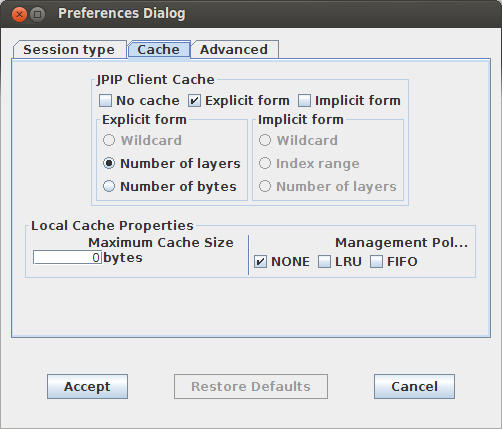
\includegraphics[scale=0.4]{images/CADIViewer-screenshot-PreferencesDialog_Cache.png} \\
\end{figure}
\vspace*{0.5cm}

Regarding the tab \emph{Advanced} in the \emph{Preferences dialog window} allows to
set detailed options of the JPIP protocol. It is not recommened to modify this options
unless you are sure about their meaning. \\
\begin{figure}[!h]
	\centering
	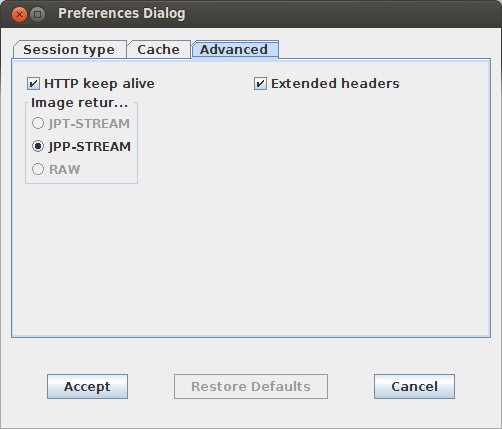
\includegraphics[scale=0.4]{images/CADIViewer-screenshot-PreferencesDialog_advanced.png} \\
\end{figure}
\vspace*{0.5cm}

The menu \emph{Edit $>$ Preferences} opens the \emph{Preferences} dialog window to
configure the logs of the application. Logs can be enabled or disables in the 
\emph{Enable} check. If enabled, it is mandatory to choose the format, the level of
detail, and the destination (console or file). \\
\begin{figure}[!h]
	\centering
	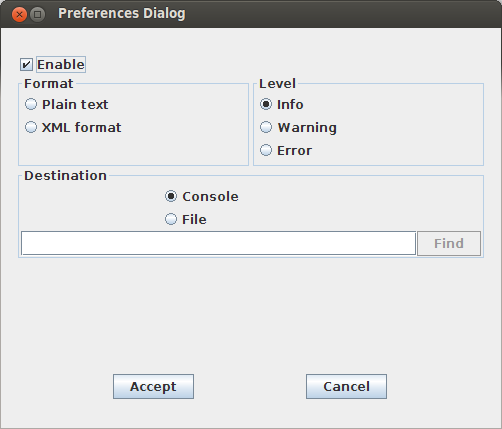
\includegraphics[scale=0.4]{images/CADIViewer-screenshot-EditPreferences.png} \\
\end{figure}



\newpage
%%%%%%%%%%%%%%%%%%%%%%%%%%%%%%%%%%%%%%%%%%%%%%%%%%%%%%%%%%%%%%%%%%%%%%%%%%%%%%%
\section{CADIProxy}
\label{sect:proxy}
The CADIProxy applications implements a JPIP proxy. It is a command line application
that not only caches all images server through the proxy but it can do prefetching.

\subsection{CADIProxy parameters}
\label{sect:proxy_parameters}

\begin{center}\begin{tabular}{|rr|rl|rl|}
\hline
\multicolumn{2}{|l|}{\textbf{$-$$-$ports}} & \multicolumn{4}{|l|}{$\{$int$[$int $[$int $[$ ...$]$$]$$]$$\}$} \\
\cline{3-6}
\multicolumn{2}{|l|}{\textbf{$-$p}} & \emph{Mandatory:} & No & \emph{Max reps:} & 1 \\
\hline
\emph{Explanation:} & \multicolumn{5}{|p{12cm}|}{Ports where server will be listening to the client requests.} \\
\hline
\emph{Default:} & \multicolumn{5}{|p{12cm}|}{8080} \\
\hline
\end{tabular}\end{center}
\begin{center}\begin{tabular}{|rr|rl|rl|}
\hline
\multicolumn{2}{|l|}{\textbf{$-$$-$numThreads}} & \multicolumn{4}{|l|}{$\{$int$\}$} \\
\cline{3-6}
\multicolumn{2}{|l|}{\textbf{$-$nt}} & \emph{Mandatory:} & No & \emph{Max reps:} & 1 \\
\hline
\emph{Explanation:} & \multicolumn{5}{|p{12cm}|}{Number of threads that will be launched to process client requests.} \\
\hline
\emph{Default:} & \multicolumn{5}{|p{12cm}|}{1} \\
\hline
\end{tabular}\end{center}
\begin{center}\begin{tabular}{|rr|rl|rl|}
\hline
\multicolumn{2}{|l|}{\textbf{$-$$-$type}} & \multicolumn{4}{|l|}{$\{$int$\}$} \\
\cline{3-6}
\multicolumn{2}{|l|}{\textbf{$-$t}} & \emph{Mandatory:} & No & \emph{Max reps:} & 1 \\
\hline
\emph{Explanation:} & \multicolumn{5}{|p{12cm}|}{Indicates the type of proxy that will be used. Allowed values are:\newline	1- transparent proxy\newline	2- cached proxy. All data transmitted from servers to clients are cached.\newline	3- cache proxy with prefetching. It is an extension of the "cached proxy" adding the capability of prefetching.\newline OBS: Option 3 can be qualified by "-pwt" or "-pm" parameters. If none of them is set, deafult options to be considered are: "-pdh=3", "-pwt=1", and "-mp=0.1" , respectively} \\
\hline
\emph{Default:} & \multicolumn{5}{|p{12cm}|}{3} \\
\hline
\end{tabular}\end{center}
\begin{center}\begin{tabular}{|rr|rl|rl|}
\hline
\multicolumn{2}{|l|}{\textbf{$-$$-$prefetchingDataHistory}} & \multicolumn{4}{|l|}{$\{$int$\}$} \\
\cline{3-6}
\multicolumn{2}{|l|}{\textbf{$-$pdh}} & \emph{Mandatory:} & No & \emph{Max reps:} & 1 \\
\hline
\emph{Explanation:} & \multicolumn{5}{|p{12cm}|}{Is the data, previous windows of interest requested, used to build the actual WOI to be prefetched. Allowed values:\newline	1- uses the history of the windows of interest requested by all clients over an image. View windows are sorted following a FIFO strategy for all clients.\newline	2- prediction of windows of interest to be downloaded are done for each client taken into account only the historic wois for that client.\newline	3- computes the prefetching woi using the lastest window of interest requested by all clients over each image.\newline 	OBS: This option can only be set when the --type parameter is 3 (cached proxy with prefetching).} \\
\hline
\emph{Default:} & \multicolumn{5}{|p{12cm}|}{3} \\
\hline
\end{tabular}\end{center}
\begin{center}\begin{tabular}{|rr|rl|rl|}
\hline
\multicolumn{2}{|l|}{\textbf{$-$$-$prefetchingWOIType}} & \multicolumn{4}{|l|}{$\{$int$\}$} \\
\cline{3-6}
\multicolumn{2}{|l|}{\textbf{$-$pwt}} & \emph{Mandatory:} & No & \emph{Max reps:} & 1 \\
\hline
\emph{Explanation:} & \multicolumn{5}{|p{12cm}|}{Allows to choose how the Windows of Interest to be prefetching is built from the historic of data. Allowed values:\newline	1- prediction of the window of interest to be prefetched  is based on weighted wois of the historic of windows of interest. Probability of movements can be modified by means of the "-mp" parameter.\newline	2- the window of interest to be prefected is the bounding box of the historic window of interest.\newline OBS: This parameter is only allowed if the "--type" parameter is 3 (cached proxy with prefetching).\newline OBS: This parameter is not compatible with the "-pm" parameter.} \\
\hline
\emph{Default:} & \multicolumn{5}{|p{12cm}|}{1} \\
\hline
\end{tabular}\end{center}
\begin{center}\begin{tabular}{|rr|rl|rl|}
\hline
\multicolumn{2}{|l|}{\textbf{$-$$-$movementProbabilities}} & \multicolumn{4}{|l|}{$\{$float float float float float float float float float float$\}$} \\
\cline{3-6}
\multicolumn{2}{|l|}{\textbf{$-$mp}} & \emph{Mandatory:} & No & \emph{Max reps:} & 1 \\
\hline
\emph{Explanation:} & \multicolumn{5}{|p{12cm}|}{Probabilities of the movements to be used by the prefetching. Values must be sorted according with the following criterion: right, up\-right, up, up\-left, left, down\-left, down, down\-right, zoom in, zoom out.\newline	 OBS: The sum of all values must be less or equal than 1.\newline	OBS: This option can only be set when the --type parameter is 3 (cached proxy with prefetching) and "-pwt" is 1.} \\
\hline
\emph{Default:} & \multicolumn{5}{|p{12cm}|}{0.1} \\
\hline
\end{tabular}\end{center}
\begin{center}\begin{tabular}{|rr|rl|rl|}
\hline
\multicolumn{2}{|l|}{\textbf{$-$$-$predictiveModel}} & \multicolumn{4}{|l|}{$\{$string$\}$} \\
\cline{3-6}
\multicolumn{2}{|l|}{\textbf{$-$pm}} & \emph{Mandatory:} & No & \emph{Max reps:} & 1 \\
\hline
\emph{Explanation:} & \multicolumn{5}{|p{12cm}|}{This parameter indicates that a predictive model, semantic information, is applied in the image delivering and prefetching. Predictive model to be applied is read from a text file located at path given by this parameter and whose name is the same as the compressed image but with the extension "pm". The file must have a line for each spatial region (precinct) with the following format "precinct\_id value", where the precinct\_id is the unique precinct identifier defined in the JPIP protocol and the value is a real number in the range [0, 1] with the relevance of the precinct. The remainder precincts not included in the file will be considered with relevance 0. And if the beginning-of-line character is an \#, it is considered a comment and ignored.\newline OBS: This parameter is only allowed if the "--type" parameter is 3 (cached proxy with prefetching).\newline OBS: This parameter is not compatible with the "-pwt" parameter.\newline OBS: If there is not a semantic file associated with an image, prefetching is done considering the option 1 of the -pwt parameter.} \\
\hline
\emph{Default:} & \multicolumn{5}{|p{12cm}|}{} \\
\hline
\end{tabular}\end{center}
\begin{center}\begin{tabular}{|rr|rl|rl|}
\hline
\multicolumn{2}{|l|}{\textbf{$-$$-$logFile}} & \multicolumn{4}{|l|}{$\{$string$\}$} \\
\cline{3-6}
\multicolumn{2}{|l|}{\textbf{$-$lf}} & \emph{Mandatory:} & No & \emph{Max reps:} & 1 \\
\hline
\emph{Explanation:} & \multicolumn{5}{|p{12cm}|}{File where logs are saved.} \\
\hline
\emph{Default:} & \multicolumn{5}{|p{12cm}|}{} \\
\hline
\end{tabular}\end{center}
\begin{center}\begin{tabular}{|rr|rl|rl|}
\hline
\multicolumn{2}{|l|}{\textbf{$-$$-$logXML}} & \multicolumn{4}{|l|}{$\{$boolean$\}$} \\
\cline{3-6}
\multicolumn{2}{|l|}{\textbf{$-$lx}} & \emph{Mandatory:} & No & \emph{Max reps:} & 1 \\
\hline
\emph{Explanation:} & \multicolumn{5}{|p{12cm}|}{XML format is used in the log file. Value is a boolean: 0 indicates simple file format is used and 1 indicates XML format is used.} \\
\hline
\emph{Default:} & \multicolumn{5}{|p{12cm}|}{0} \\
\hline
\end{tabular}\end{center}
\begin{center}\begin{tabular}{|rr|rl|rl|}
\hline
\multicolumn{2}{|l|}{\textbf{$-$$-$logEnabled}} & \multicolumn{4}{|l|}{$\{$boolean$\}$} \\
\cline{3-6}
\multicolumn{2}{|l|}{\textbf{$-$le}} & \emph{Mandatory:} & No & \emph{Max reps:} & 1 \\
\hline
\emph{Explanation:} & \multicolumn{5}{|p{12cm}|}{Enables or disables the log. See the "-ll" parameter for more information about the detail level of logs.} \\
\hline
\emph{Default:} & \multicolumn{5}{|p{12cm}|}{} \\
\hline
\end{tabular}\end{center}
\begin{center}\begin{tabular}{|rr|rl|rl|}
\hline
\multicolumn{2}{|l|}{\textbf{$-$$-$logLevel}} & \multicolumn{4}{|l|}{$\{$int$\}$} \\
\cline{3-6}
\multicolumn{2}{|l|}{\textbf{$-$ll}} & \emph{Mandatory:} & No & \emph{Max reps:} & 1 \\
\hline
\emph{Explanation:} & \multicolumn{5}{|p{12cm}|}{Is the severity of the messages which will be logged. The "-le" parameter is set automatically. Available values are:\newline	2- logs informative messages\newline	3- logs warning messages\newline	4- logs error messages\newline when a log level is set, all upper levels are automatically set but lower severity messages are filtered.} \\
\hline
\emph{Default:} & \multicolumn{5}{|p{12cm}|}{2} \\
\hline
\end{tabular}\end{center}
\begin{center}\begin{tabular}{|rr|rl|rl|}
\hline
\multicolumn{2}{|l|}{\textbf{$-$$-$cacheDirectory}} & \multicolumn{4}{|l|}{$\{$string$\}$} \\
\cline{3-6}
\multicolumn{2}{|l|}{\textbf{$-$cd}} & \emph{Mandatory:} & No & \emph{Max reps:} & 1 \\
\hline
\emph{Explanation:} & \multicolumn{5}{|p{12cm}|}{Directory used as a temporal directory to save the cache data (not implemented yet).} \\
\hline
\emph{Default:} & \multicolumn{5}{|p{12cm}|}{} \\
\hline
\end{tabular}\end{center}
\begin{center}\begin{tabular}{|rr|rl|rl|}
\hline
\multicolumn{2}{|l|}{\textbf{$-$$-$maxRate}} & \multicolumn{4}{|l|}{$\{$int$\}$} \\
\cline{3-6}
\multicolumn{2}{|l|}{\textbf{$-$mr}} & \emph{Mandatory:} & No & \emph{Max reps:} & 1 \\
\hline
\emph{Explanation:} & \multicolumn{5}{|p{12cm}|}{Specifies the maximum rate (bytes per second) which will be used to delivery data (0 means unlimited).} \\
\hline
\emph{Default:} & \multicolumn{5}{|p{12cm}|}{0} \\
\hline
\end{tabular}\end{center}
\begin{center}\begin{tabular}{|rr|rl|rl|}
\hline
\multicolumn{2}{|l|}{\textbf{$-$$-$trafficShaping}} & \multicolumn{4}{|l|}{$\{$int$\}$} \\
\cline{3-6}
\multicolumn{2}{|l|}{\textbf{$-$ts}} & \emph{Mandatory:} & No & \emph{Max reps:} & 1 \\
\hline
\emph{Explanation:} & \multicolumn{5}{|p{12cm}|}{Allows to choose a trafic shaping algorithm. Allowed values are:	0- None algoritm is applied.	1- The token-bucket algoritm is applied. Data are transmitted at the constant rate fixed by the "-mr" parameter rate, but it also allows data busts.	2- The leaky-bucket algoritm is applied. Data are delivered at the constant rate defined in the "-mr" option.OBS: This parameter requires the "-mr" parameter.} \\
\hline
\emph{Default:} & \multicolumn{5}{|p{12cm}|}{0} \\
\hline
\end{tabular}\end{center}
\begin{center}\begin{tabular}{|rr|rl|rl|}
\hline
\multicolumn{2}{|l|}{\textbf{$-$$-$help}} & \multicolumn{4}{|l|}{} \\
\cline{3-6}
\multicolumn{2}{|l|}{\textbf{$-$h}} & \emph{Mandatory:} & No & \emph{Max reps:} & 1 \\
\hline
\emph{Explanation:} & \multicolumn{5}{|p{12cm}|}{Displays this help and exits program.} \\
\hline
\emph{Default:} & \multicolumn{5}{|p{12cm}|}{} \\
\hline
\end{tabular}\end{center}
\begin{center}\begin{tabular}{|rr|rl|rl|}
\hline
\multicolumn{2}{|l|}{\textbf{$-$$-$warranty}} & \multicolumn{4}{|l|}{} \\
\cline{3-6}
\multicolumn{2}{|l|}{\textbf{$-$w}} & \emph{Mandatory:} & No & \emph{Max reps:} & 1 \\
\hline
\emph{Explanation:} & \multicolumn{5}{|p{12cm}|}{} \\
\hline
\emph{Default:} & \multicolumn{5}{|p{12cm}|}{} \\
\hline
\end{tabular}\end{center}
\begin{center}\begin{tabular}{|rr|rl|rl|}
\hline
\multicolumn{2}{|l|}{\textbf{$-$$-$liability}} & \multicolumn{4}{|l|}{} \\
\cline{3-6}
\multicolumn{2}{|l|}{\textbf{$-$l}} & \emph{Mandatory:} & No & \emph{Max reps:} & 1 \\
\hline
\emph{Explanation:} & \multicolumn{5}{|p{12cm}|}{} \\
\hline
\emph{Default:} & \multicolumn{5}{|p{12cm}|}{} \\
\hline
\end{tabular}\end{center}
\begin{center}\begin{tabular}{|rr|rl|rl|}
\hline
\multicolumn{2}{|l|}{\textbf{$-$$-$copyright}} & \multicolumn{4}{|l|}{} \\
\cline{3-6}
\multicolumn{2}{|l|}{\textbf{$-$c}} & \emph{Mandatory:} & No & \emph{Max reps:} & 1 \\
\hline
\emph{Explanation:} & \multicolumn{5}{|p{12cm}|}{} \\
\hline
\emph{Default:} & \multicolumn{5}{|p{12cm}|}{} \\
\hline
\end{tabular}\end{center}


\newpage
%%%%%%%%%%%%%%%%%%%%%%%%%%%%%%%%%%%%%%%%%%%%%%%%%%%%%%%%%%%%%%%%%%%%%%%%%%%%%%%
\subsection{Examples}
\label{sect:proxy_examples}

In this section all supported parameters for the server command line are explained.
For a detailed description of each element in the table displayed for each parameter,
please see \ref{sect:annex_parameters}.


\begin{itemize}

	\item Launch the JPIP proxy with the defualt options. Thus, the proxy is running on port 8080, it uses as number of threads as number of processors, and it is configure to work on prefetching mode with all the movements equally likely.
	\begin{framed}
	\texttt{\$java -jar dist/CADIProxy.jar -h}
	\end{framed}

	\item Display the help information.
	\begin{framed}
	\texttt{\$java -jar dist/CADIProxy.jar -h}
	\end{framed}
	
	\item Proxy working as a transparent proxy.
	\begin{framed}
	\texttt{\$java -jar dist/CADIProxy.jar -t 1}
	\end{framed}
	
	\item Proxy working in \emph{cache mode}.
	\begin{framed}
	\texttt{\$java -jar dist/CADIProxy.jar -t 2}
	\end{framed}
	
	\item Proxy in prefethcing mode. Proxy is configured to do prefetching using as historic the lastest Window of Interest requested by all clients over each image and predicting the region to the image to be requested as a weigthing of the historic. Probabilities used to compute the next potential region are the same for all the movements (0.1).
	\begin{framed}
	\texttt{\$java -jar dist/CADIProxy.jar -t 3 -pdh 3 -pwt 1}
	\end{framed}
	
	\item This example is the same as the previous one, but in this case the probabilities used to compute the next potential region of the image to be requested have been set to 0.075 for the panning movements and 0.2 for the zooms.
	\begin{framed}
	\texttt{\$java -jar dist/CADIProxy.jar -t 3 -pdh 3 -pwt 1 -mp 0.075 0.075 0.075 0.075.075 0.075 0.075 0.075  0.2 0.2}
	\end{framed}
	
	\item Proxy is configure to work as a prefetching proxy using the predictive model qualifier to compute the next potential region to be requested. Files containing the semantic information about images are in the \emph{pred\_models} directory.
	\begin{framed}
	\texttt{\$java -jar dist/CADIProxy.jar -t 3 -pdh 3 -pm pred\_models/}
	\end{framed}
	
	
\end{itemize}


\newpage
%%%%%%%%%%%%%%%%%%%%%%%%%%%%%%%%%%%%%%%%%%%%%%%%%%%%%%%%%%%%%%%%%%%%%%%%%%%%%%%

\section*{Annex: Parameters description}
\label{sect:annex_parameters}
Parameters have two formats: the long and the short
specification. Long specification has $-$$-$ at the beginning while
short specification has $-$ (it does not matter which one you
choose). Each parameter has its own arguments, which usually are
integers, floats, booleans (0 to indicate false and 1 to indicate
true) or strings. If the user specifies some invalid arguments, the
application will display warning messages. Most of these parameters
are not mandatory. When they are not specified default values are
used. The following table shows how each parameter will be
displayed in this manual: 

\begin{center}\begin{tabular}{|rr|rlrl|}
	 \hline
	 \multicolumn{2}{|l|}{\textbf{$-$$-$longParameter}} &
	 \multicolumn{4}{|l|}{$\{$parameter arguments$\}$} \\
	 \cline{3-6}
	 \multicolumn{2}{|l|}{\textbf{$-$shortParameter}} & \emph{Mandatory:} & Yes/No & &  \\
	 \hline
	 \emph{Explanation:} & \multicolumn{5}{|p{12cm}|}{Parameter explanation} \\
	 \hline
	 \emph{Default:} & \multicolumn{5}{|p{12cm}|}{Parameter default values.} \\
	 \hline
\end{tabular}\end{center}

\newpage
%%%%%%%%%%%%%%%%%%%%%%%%%%%%%%%%%%%%%%%%%%%%%%%%%%%%%%%%%%%%%%%%%%%%%%%%%%%%%%%

\section*{Annex: Requirements}
\label{sect:annex}

\subsection*{Libraries}
\label{ssect:annex_libraries}

CADISoftware only needs the JRE version 1.6 or higher to run.


\subsection*{Compilation}
\label{ssect:annex_compilation}

Compile the CADISoftware is easy because there is a \emph{build.xml} file ready to compile the project. The binaries of the complied project will be in the \emph{dist/} directory. It must be noted that the Java Advanced Imaging (JAI) is necessary to compile the source code.


\subsection*{JVM parameters}
\label{ssect:annex_jvm}

The amount of memory depends on the CADI Software application. Thus, the memory requirements of CADIServer are low and they will depend on the number of images being served because it only works with a indexed image. However, in the CADIClient or CADIViewer the amount of memory depends on the dimensions of the image region to be decoded, the larger is the region the more memory is needed. And regarding the CADIProxy, it gathers both requirements of CADIServer and CADIClient.

In order to avoid a Java Heap Memory error when CADISoftware is run, it is recommended to set the maximum amount of memory that the application can allocate via the \emph{-Xmx} parameter of the JVM, i.e. \emph{java -Xmx1024m -jar dist/CADIServer.jar}.


\end{document}
